\documentclass[paper=a4,fontsize=11pt]{report} % A4 paper and 11pt font size

\usepackage[T1]{fontenc} % Use 8-bit encoding that has 256 glyphs
\usepackage{fourier} % Use the Adobe Utopia font for the document - comment this line to return to the LaTeX default
\usepackage{graphicx} % For pictures
\usepackage{booktabs} % For tables
\usepackage{tabularx} % For tables
\usepackage{hyperref}
\usepackage[english]{babel} % English language/hyphenation
\usepackage{amsmath,amsfonts,amsthm} % Math packages

\usepackage[margin=1.5in]{geometry}

\usepackage{lipsum} % Used for inserting dummy 'Lorem ipsum' text into the template

\usepackage{sectsty} % Allows customizing section commands
\allsectionsfont{\centering \normalfont\scshape} % Make all sections centered, the default font and small caps

\usepackage{fancyhdr} % Custom headers and footers
\pagestyle{fancyplain} % Makes all pages in the document conform to the custom headers and footers
\fancyhead{} % No page header - if you want one, create it in the same way as the footers below
\fancyfoot[L]{} % Empty left footer
\fancyfoot[C]{} % Empty center footer
\fancyfoot[R]{\thepage} % Page numbering for right footer
\renewcommand{\headrulewidth}{0pt} % Remove header underlines
\renewcommand{\footrulewidth}{0pt} % Remove footer underlines
\setlength{\headheight}{13.6pt} % Customize the height of the header

\numberwithin{equation}{section} % Number equations within sections (i.e. 1.1, 1.2, 2.1, 2.2 instead of 1, 2, 3, 4)
\numberwithin{figure}{section} % Number figures within sections (i.e. 1.1, 1.2, 2.1, 2.2 instead of 1, 2, 3, 4)
\numberwithin{table}{section} % Number tables within sections (i.e. 1.1, 1.2, 2.1, 2.2 instead of 1, 2, 3, 4)

% \setlength\parindent{0pt} % Removes all indentation from paragraphs - comment this line for an assignment with lots of text

\renewcommand{\thesection}{\arabic{section}}

%----------------------------------------------------------------------------------------
%	TITLE SECTION
%----------------------------------------------------------------------------------------

\newcommand{\horrule}[1]{\rule{\linewidth}{#1}} % Create horizontal rule command with 1 argument of height

\title{	
\normalfont \normalsize 
\textsc{Georgia Institute of Technology} \\ [25pt] % Your university, school and/or department name(s)
\horrule{0.5pt} \\[0.4cm] % Thin top horizontal rule
\huge CS 6210 Project 4 Report: GTStore \\ % The assignment title
\horrule{2pt} \\[0.5cm] % Thick bottom horizontal rule
}

\author{Manas George, Paras Jain} % Your name

\date{\normalsize\today} % Today's date or a custom date

\begin{document}

\maketitle % Print the title

\section{Partitioning}
\label{partitioning}
\subsection{Design notes}
We utilize a consistent hashing strategy\footnote{\url{http://michaelnielsen.org/blog/consistent-hashing/}} that is resilient to the addition and removal of nodes. A hash indicates a position on a virtual ring upon which nodes lie. Following the ring to the nearest node allows reaching the node or an adjacent node in the case of changing cluster membership. Each node gets a random value in this space representing position on the ring. Each data item is assigned to a node by hashing the client ID concatenated with the key to get its position on the ring, and assigning it to the first node with a position larger than the item's position.

When the client determines which partition and node their data is allocated to, it contacts said node. In case of failure (e.g. coordinating node is down) the client proceeds to query subsequent nodes around the ring. In this way, arrival or departure of nodes only affects immediate neighbours. We assume homogenous nodes and accept the cost of non-uniform data and load distribution that results from the randomized position assignment. This issue is not significant as MD5 has a roughly even distribution across the hash space\footnote{\url{http://michiel.buddingh.eu/distribution-of-hash-values}}.

\subsection{Discussion}
This design works very well in practice. Large scale services like Akamai utilize consistent hashing at a global scale and it proves quite resilient to node failure. This is a very desirable property in our system. We have gone beyond the suggested design and used the structure of the ring to increase availability by cycling through adjacent nodes if the primary hash result is down. Furthermore, because the hash is calculated using both the client id and the supplied key, no single set of nodes is responsible for a single client's data, which helps easily spread out the load of all of the clients across all of the nodes, allowing us to scale easily. An alternate scheme in which a single set of nodes is consistently assigned to the same client would result in some nodes seeing more traffic than others, potentially imposing huge scaling costs on some clients. 

However, there are some potential drawbacks of this strategy. One notable limitation is a cap on the number of servers that can be added to the ring. As of now, we cap the maximum size of the ring. In order to increase capacity further, we would have to allocate a new hash ring and reallocate servers onto the ring. This can be an expensive operation. Another drawback is performance - unlike hashing strategies (such as those that rely on modular arithmetic over primes), this strategy is not constant time. Realistically, this turns out to not be a major limitation for our service as the ring is not sized too large which limits the maximum amount of time a hash operation could take.

\section{Replication}
\subsection{Design notes}
Data is replicated upon a \texttt{put} operation. When a client sends a request to the client library, the request will be routed to the coordinating server for the write as dictated by the consistent hashing strategy, as described in Section \ref{partitioning}. The coordinating server will contact the next $R$ nodes in the ring. If $W$ of these writes succeed, then the operation is marked as a success. This strategy has the client delegate one DataNode as the coordinator of the request, where that coordinating DataNode will communicate internally to its peers. The Manager keeps track of membership, modifying the membership lists of each data node appropriately when leaving/additional nodes are detected.

\subsection{Replication factors}
By default, we use the following replication factors:
\begin{enumerate}
\item Data is replicated 3 times on write. Writes are deemed successful if at least 2 of these attempts succeed.
\item Data is read 3 times on read. Reads are deemed successful if at least 2 of these attempts succeed. Note that this number is before conflicts are resolved.
\end{enumerate}

This ensures that the property $W + R > K$ where $K$ is the replication factor. Thus, writes and reads will need a majority of successes to succeed.

\subsection{Discussion}
The design discussed here has several benefits. The client has a single point of contact during the operation and the DataNodes can then communicate internally on a separate high speed network. This is done in order to minimize traffic between clients and data nodes, restricting that purely to transfer of data. There is also the assumption that the data nodes have more processing power available to them than the clients and therefore should do more of the work.

There are some tradeoffs, however. With only 3 replicas, we can only tolerate one node failure while ensuring availability. This number should be odd to ensure that there is some majority in the system. Given the properties of the ring, we can also get into situations where sequences of node failures and recoveries could potentially disrupt system wide consistency. However, these patterns are likely to be rare and are difficult to recover from regardless.

Failure of the node with the primary replica is no more or less catastrophic than failure of any other node; quorum is still maintained as long as the other replicas are alive and the data is still available. Our partitioning scheme ensures that clients simply contact the next node in the ring if the primary replica is down; under our replication scheme, this is simply the secondary replica, which will usually be able to contact the third replica and obtain enough copies to satisfy quorum, thus satisfying the get request.

Replication is bounded in time, parameterized by the factor $W$. Increasing this increases the maximum amount of time replication takes, and vice versa. Empirically, triplicate replication seems to work well in practice, providing a good trade off between latency and reiliability.

\section{Consistency}

\subsection{Design notes}
We based our versioning strategy off the vector clock method described in the Dynamo paper. This strategy is eventually consistent, meaning that there is an upper bound on propagation times given no failures. A single put call returns before the update is applied on all replicas. We treat modifications to data item as a new, immutable version; multiple versions of a data item may be present in the system at any given point of time. Thus, we are able to write anytime to the system. This necessitates a consistency resolution protocol at the time of read.

This consistency problem is solved using vector clocks. These clocks are lists of \texttt{(node, version)} tuples that store the versioning information across branches. This allows the system to trace though the lineage of a key-value pair and attempt to resolve consistency issues within the system. In the case that consistency issues cannot be resolved, we return a set of maximal items (from the partially-order set of results) to the client and allow them to resolve the conflict in the \texttt{ConflictSet}. The client can register a callback handler which will resolve any issues.

When issues are resolved, the subsequent put is treted as the final version of the data item. We effectively push the responsibility of reconciliation in such cases to the user. If ordering is possible, we pick the latest version. 

\subsection{Discussion}
There are numerous benefits to this approach. We can resolve most consistency issues within the system without additional information from the client using the vector clocks. The small number of conflicts otherwise that need to be resoved can be handled within the client. This approach allows us to relax consistency while still being able to recover state. This approach also affords us write availability at the cost of read consistency.

A major drawback is the large storage requirements presented by vector clocks. Over time, these clocks could grow to be bigger than the original data that was being stored. Garbage collection can be a technique used to recover wasted space. We have not implemented clock truncation yet, so we assume that there aren't multiple catastrophic server failures. We ignore this problem as this issue would be difficult to recover from in any distributed system.


\section{Put/Get operations}
We now walk though what happens when a put and get operation occurs.

\begin{enumerate}
\item We store key value pairs, both of which are blobs of bytes. The key is MD5 hashed after prepending the client ID to it, borrowing a trick from the Dynamo paper, in order to get an unique identifier that is used for all internal operations. This hash distribution is relatively even across the hash space.
\item The client determines which node to send get/put requests to based on the hash as described in Section \ref{partitioning}.
\item For put requests, the node generates the vector clock for the new version and writes the new version locally. It then sends the new version to the two successor nodes on the ring. The write is considered successful if one replica responds, which is a majority (the coordinator itself and the other replica).
\item For get requests, the node asks the two ring successor nodes for all existing versions of the data and waits for both to respond before reconciling and returning the result. If reconciliation takes place, the reconciled versions are written back into the replication nodes.
\item If multiple leaves are returned, the client generates an unresolved \texttt{ConflictSet}. The client then uses the conflict resolution handler that the client sets at runtime to solve for which leaf is relevant. This value is then written back to the store as the latest version.
\end{enumerate}


\section{Temporary Failures}
Borrowing a technique from the Dynamo paper, if a put operation detects that one of the nodes it tries to write to is unavailable, it moves on to the next node in the ring, marking it as a ``hinted'' write. Hinted writes are stored separately in the data nodes, and when the failed node comes back online, the Manager asks all nodes to write stored false writes back to their intended locations. We assume low membership churn and that node failures are transient, and do not implement measures to deal with permanent node failures.

The Manager node periodically contacts DataNodes (10 second heartbeat) in order to calculate membership information and inform other DataNodes when a previously failed node has come back online, or if a DataNode has left the ring. In the case of one-off permanent failures, neighbouring nodes pick up the slack and the leeway allowed by the replication mechanism ensures that data is not lost permanently, as long as failures are not catastrophic. 


\section{Design tradeoff analysis}
We have already discussed design tradeoffs in the context of Partition, Replication and Versioning strategies. We now discuss tradeoffs related to our decision to prioritize performance and scalability. Our goal was to design the system to have linear scalability -- as we add more nodes, we wanted throughput to scale. This decision impacted many choices thoughout our design. Consistent hashing is critical to this design choice as it allows arbitrary addition and removal of nodes with stable partitioning. This also impacted our replication strategy as we decided handle replication internally between DataNodes. This reduced client-DataNode chatter as we assumed that DataNodes would be hosted on more powerful servers with fast interconnect between peer DataNodes. This also caused us to opt for a semi-distributed organization of DataNode responsibilities. All DataNodes are equal peers - no server has more or less responsiblity (with exception of the leader). Thus, every DataNode can coordinate replication for its own keys. This prevents there being a single bottleneck though one node.\footnote{The master still is a bottleneck for the system but it is performing much less work per RPC than the DataNode.}

We also chose to resolve conflicts in the client. This choice was motivated by two factors - first was to empower the client to resolve conflicts with more local information, and second was to reduce reconciliation load from the DataNodes. Clients recieve results in a \texttt{ConflictSet} batch and resolve the conflicts locally on their node, which is an $O(n^2)$ operation. As it more than linear, we chose to offload this responsibility to the client. This also improved the power of conflict resolution
strategies.

These choices paid off in the end. As my machine is a laptop, I only tested running up to 5 DataNodes. As I scaled from 3 to 5 DataNodes, we indeed see system throughput increases linearly. This was exactly what we were working towards.

\noindent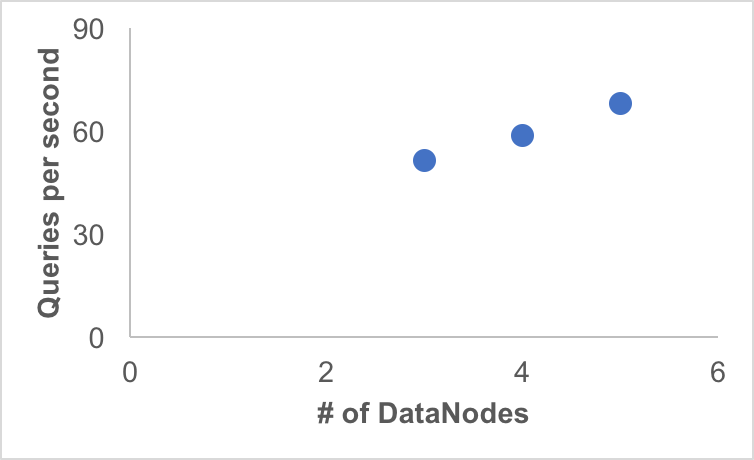
\includegraphics[width=.65\textwidth]{LinearScaling.png}

We see that as we add new nodes, the throughput scales as well. This is a useful property in a distributed hash table as it allows increasing system throughput by horizontally scaling over time. We can add new nodes gradually to meet demand.

\subsection{Analyzing impact of failure on throughput}
We wanted to examine the performance of our system with failure. In a cluster of 7 DataNodes, we rebooted a single DataNode once at iteration 20 and once just after iteration 32. We saw throughput drop immediately, which is expected. However, performance quickly normalizes to the baseline after each failure.\\

\noindent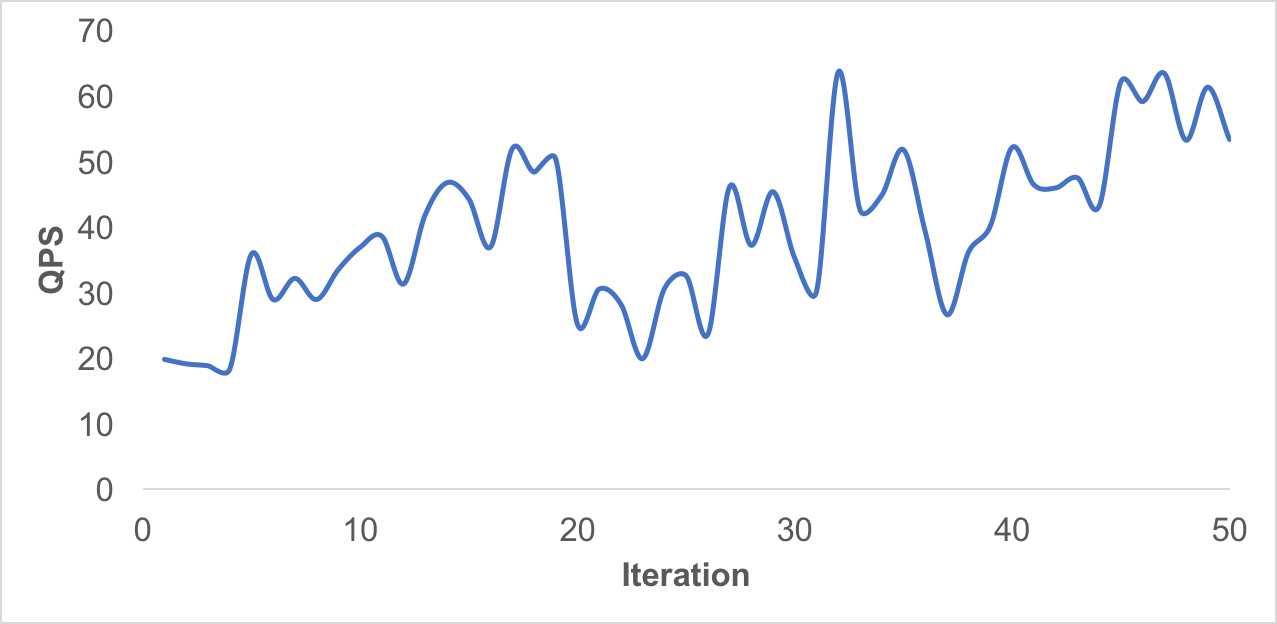
\includegraphics[width=\textwidth]{throughput_failiure.png}

This behavior is another helpful factor for a distributed hash table. In a production deployment, a customer can overprovision the cluster so that temporary failures will not disrupt overall system health. As nodes recover, system throughput recovers as well.

\end{document}
